\section {Molecular Orientation}

Understanding the orientation of succinic acid molecules helps us understand the chemistry taking place, and to interpret our experimental results. To build a clearer image of how succinic acid orients throughout the water interface, we have calculated bivariate angular distributions to define molecular orientation at various depths in the water surface. Figure \ref{fig:angle-definitions} depicts the succinic acid molecule and shows two angle definitions relative to the surface normal vector (labeled ``z'') that are used to define the molecular orientation. The angular tilt, $\theta$, is an angle between the O-C-O bisector axis of the carboxylic acid head group (pointing from the carbon to the oxygen end) and the vector normal to the plane of the water surface. $\theta$ varies from being aligned with the surface normal ($\theta=0$\textdegree), to perpendicular and in the plane of the surface ($\theta=90$\textdegree), to anti-aligned with the surface normal ($\theta=180$\textdegree) pointing in towards the water bulk. 

The carboxylic acid group twist angle, $\phi$, measures the angle between the plane formed by the O-C-O atoms of the carboxylic acid, and the plane formed by the O-C-O bisector and the surface normal vectors. This is a dihedral angle defined by the following three vectors: 1) surface normal (``z''), 2) the O-C-O bisector axis, 3) and the carbonyl C-O$_{carb}$ bond-vector of the acid group. Because of the symmetry of rotations about the carboxylic acid O-C-O bisector axis with respect to the plane of the water surface, $\phi$ has a range of 0\textdegree $ \le \phi \le $180\textdegree. If $\phi=0$\textdegree the carbonyl C-O$_{carb}$ bond-vector is aligned in a plane perpendicular to the water surface, and pointing out of the surface away from the water bulk. Consequently, this same orientation causes the carbonyl C-O$_{alc}$ bond to point towards the water bulk, in the same plane. A twist of $\phi=90$\textdegree places both the O$_{carb}$ and O$_{alc}$ in the same plane, parallel to the water surface. $\phi=180$\textdegree aligns the O-C-O plane similarly to $\phi=0$\textdegree, but with the carbonyl C-O$_{alc}$ bond pointing out from the water surface, and the carbonyl C-O$_{carb}$ pointing in towards the water bulk. 

\begin{figure}[h!]
	\begin{center}
		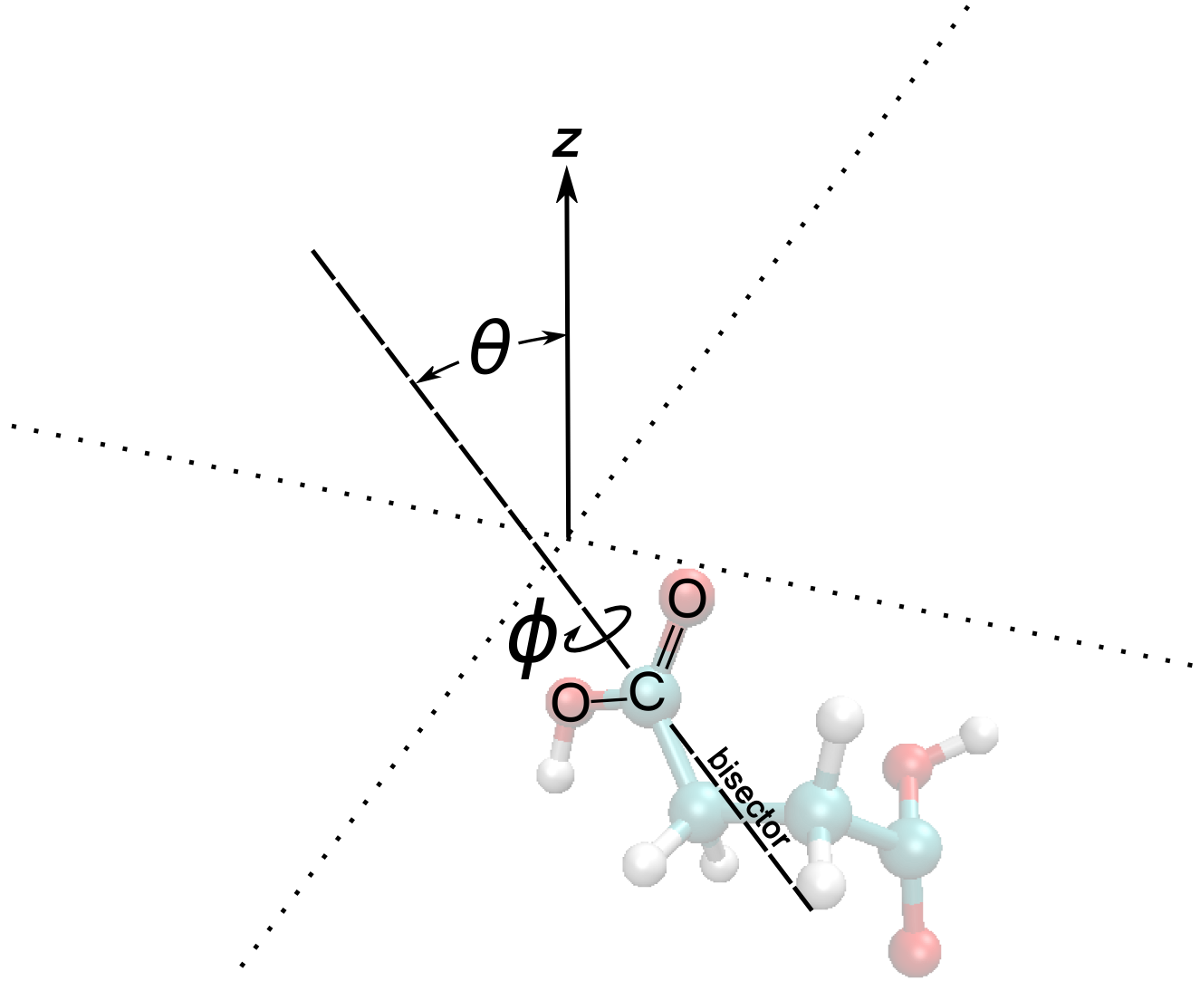
\includegraphics[scale=1.0]{images/bond-angles/bond-angle-definitions-small.png}
		\caption{Two angle definitions that characterize the carboxylic acid head group orientation relative to the water surface. The acid tilt, $\theta$, measures an angle formed between the O-C-O bisector axis of the acid group, and the vector normal to the plane of the water surface. Acid twist, $\phi$, is calculated as a dihedral formed by three vectors: the vector normal to the water surface, the O-C-O acid group bisector vector, and the vector pointing from the carbonyl carbon to the carbonyl oxygen. This is equivalent to a rotation angle about the bisector axis, referenced to an orientation with the O-C-O plane perpendicular to the water surface. $\phi = 0$\textdegree results from the carbonyl oxygen pointing further out towards the gas phase than the alcohol oxygen.}
		\label{fig:angle-definitions}
	\end{center}
\end{figure}

A third angle, $\psi$ (not shown), is the dihedral angle of the carbon backbone, where $\psi = 0$\textdegree turns the succinic acid into a ``trans-'' carbon-chain configuration. Symmetry of rotations limits the range of dihedral twists to 0\textdegree $\le \psi \le$ 180\textdegree.

Figure \ref{fig:dihedral} is an angular depth profile of the dihedral angle, $\psi$, on the y-axis, plotted against the distance of the molecular center of mass to the water surface, on the x-axis. Positions further into the water bulk appear on the left of the plot. The coloration ranges from dark blue to red, indicating low and high intensities of the 2D histogram, respectively. The greatest contribution is from the gauche configure of the acid groups. Clearly the molecule mostly has a $\psi$ value centered at 60\textdegree at all depths, as indicated by the bright red streak running horizontally across the plot, centered at $\psi=60$\textdegree. There are minor contributions from the cis-configuration of the carbon backbone at $\psi = 180$\textdegree. The $180$\textdegree configuration is represented throughout the deeper regions of the interface and in the water bulk. Near -2\angs~and further towards the surface near 0\angs, the distribution completely shifts to the $60$\textdegree gauche configuration. The succinic acid molecules within approximately 2\angs of the surface location have a strong preference for a gauche dihedral configuration. 


\begin{figure}[h!]
	\begin{center}
		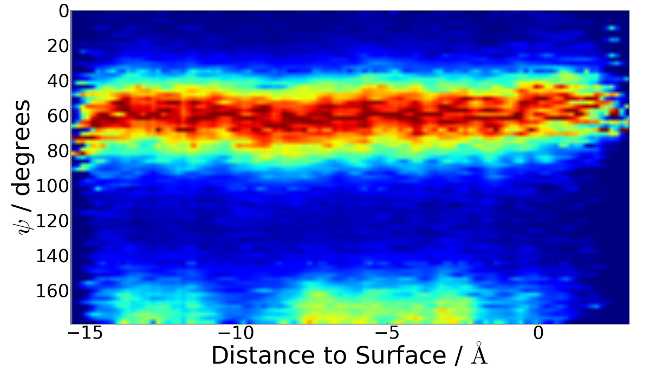
\includegraphics[scale=1.0]{images/dihedral/dihedral-small.png}
		\caption{The dihedral angle of the carbon backbone of the succinic acid molecule is found in either a gauche or cis- configuration. This angular depth profile shows the distribution of $\psi$ at different positions within the water interface. Dark blue and bright red coloration indicate low and high intensities of the histogram, respectively. The long streak of red centerd at $\psi=60$\textdegree shows the preference of the molecule to take on a gauche configuration throughout all depths from the water surface.}
		\label{fig:dihedral}
	\end{center}
\end{figure}



The acid group orientation distribution is depicted in Figure \ref{fig:carbonyl-theta-phi} at various depths throughout the interfacial water region. The plots each represent the bivariate $\theta$-$\phi$ distributions within a thin slice of the interface at a specific depth (labeled on each axis in the upper right). Negative positions are further into the water bulk, and positive depths are in the gas phase. The 0\angs~position is the water surface location as calculated through an averaging process of the positions of the outer-most waters of the slab. The areas of the distributions colored red are higher in intensity, and blue denotes low intensity. Uniform coloration indicates isotropic orientational behavior of the two angles depicted.

Beginning at 2\angs~above the water surface, all those succinic acids that reside above the water surface location have a narrow orientational range in both $\theta$ and $\phi$. We see that the intensity in the topmost plot is centered around $\theta=135$\textdegree, and $\phi$ concentrates in the 0-90\textdegree~range. This results from acid moieties that have their bisectors pointing mostly 45\textdegree~in towards the water bulk, and with the C-O$_{carb}$ directed either slightly out towards the gas phase (i.e. C-O$_{alc}$ points in towards the water bulk), or both C-O bonds align similarly with respect to the water surface. The intensity of this narrow orientational distribution increases at the 0\angs~depth, and the carboxylic oxygens remain pointing in towards the water bulk.

Moving just below the surface (-2\angs) we see the colored region shift to the center of the plot, indicating a carboxylic group that is both tilted parallel to the plane of the water surface, and also lying flat in the plane. This behavior is not altered at -4\angs, but the intensity of the orientational preference is reduced (i.e. there is less intense and more uniform coloration). At -6\angs and below into the water surface, the $\phi$ and $\theta$ distributions are isotropic.

% Tilt/Twist
\begin{figure}[h!]
	\begin{center}
		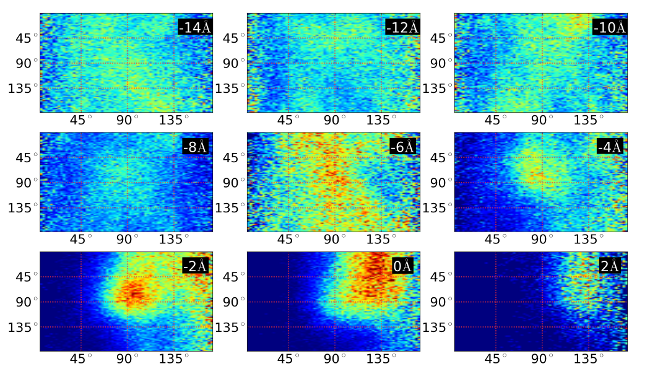
\includegraphics[scale=1.0]{images/bond-angles/carbonyl-theta-phi.png}
		\caption{The tilt and twist distributions of the carboxylic acid headgroups of the succinic acid ($\theta$ and $\phi$, respectively) characterize the orientation of the acid moiety relative to the water surface. Shown are several two-dimensional histograms of $\phi$ vs $\theta$ calculated at different depths of the interface (shown at the upper right of each axis). The depth value is calculed from the succinic acid molecular center of mass.} 
		\label{fig:carbonyl-theta-phi}
	\end{center}
\end{figure}



